\documentclass[12pt]{article}
\usepackage{verbatim}
\usepackage{graphicx}
\usepackage{amsmath}
\usepackage{parskip}
\usepackage[utf8]{inputenc}
\usepackage[T1]{fontenc}
\usepackage{lmodern}
\usepackage{color}
\usepackage{hyperref}
\usepackage{amsmath}
\usepackage{amsfonts}
\usepackage[table]{xcolor}
\usepackage{float}
\usepackage[framed, numbered]{mcode}
\usepackage[margin=3cm]{geometry}
\usepackage{subfig}
\usepackage[numbers]{natbib}
\usepackage{diagbox}

\hypersetup{
        hidelinks
}

\lstset{basicstyle=\fontsize{9}{12}\ttfamily}

\begin{document}

\title{Machine Learning in Network Biology\\Homework 1}
\author{
    Dr. Amin Emad \\ \\
    Gian Favero: 261157396 \\
}
\date{October 6th, 2023}
\maketitle
\newpage

\tableofcontents
\newpage

\section{Introduction}
Transcriptomic data refers to a collection of RNA molecules, or transcripts, present in cell tissues at a reference time. Typically, these molecules are generated in a cell through the process of transcription of DNA into RNA. This data contains insights into the expression levels of genes in a cell which can be used to predict various items like disease, stimuli response, and development, among others \cite{noauthor_transcriptome_nodate}.

Several classical machine learning approaches can be used when analyzing transcriptomic data. These include dimensionality reduction, clustering, and regression. All three of these particular approaches will be explored in this assignment using popular Python libraries to gain some insight into the data provided. Gene expression data was provided alongside this assignment(\verb|gdsc_expr_postCB.csv|) and drug response data (\verb|gdsc_dr.csv|).

\section{Part 1: Dimensionality Reduction}
Dimensionality reduction is a technique used to reduce the number of features in a dataset. This is done by projecting the data onto a lower dimensional space and finding a new, simpler set of features that can be used to represent the original data. Memory usage, computational efficiency, and visualization are all advantages of dimensionality reduction.

Several dimensionality reduction techniques are explored in this assignment. These include Principal Component Analysis (PCA), UMAP, and t-SNE algorithms.

\begin{comment}
\subsection{Theory}
\subsubsection{Principal Component Analysis}
The following is adapted from Goodfellow et al. \cite{GoodBengCour16}.

For a set of \textit{m} data points $\textbf{x}^{(i)}$ $\in$ $\mathbb{R}^n$, PCA finds a lower dimensional representation of the data by representing it as a code vector $\textbf{c}^{(i)}$ $\in$ $\mathbb{R}^l$ where $l < n$. The goal of PCA is to find a function $f$ such that $\textbf{c}^{(i)}$ = $f(\textbf{x}^{(i)})$ and a decoding function $g$ which provides $\textbf{x} \approx g(f(\textbf{x}))$. This is simply done using a decoding matrix, $\textbf{D} \in \mathbb{R}^{n \times l}$ which has columns that are orthogonal and have a unit norm. Following this, the code vector is given by:
\begin{align*}
    \textbf{c} = f(\textbf{x}) = \textbf{D}^T\textbf{x}
\end{align*}
and the reconstructed input is given by:
\begin{align*}
    \textbf{x} \approx g(\textbf{c}) = \textbf{D}\textbf{D}^T\textbf{x}
\end{align*} 

Using a closed-form or numerical optimization method, the decoding matrix can be found by minimizing the reconstruction error, $||\textbf{x} - \textbf{D}\textbf{D}^T\textbf{x}||_2^2$ across each point in the dataset.
 
$l$ is typically the only parameter selected by the user. For visual purposes, $l$ is typically chosen as 2 such that the compressed data can be plotted on a Cartesian plane.

\subsubsection{t-SNE}
t-SNE was proposed by Van der Maaten et al. \cite{vanDerMaaten2008} as a technique for visualizing high-dimensional data. At a high-level, the algorithm maps each data point to a location on a 2D or 3D map that can reveal the structure at many scales. The resulting map effectively reveals low-dimensional manifolds on which the data points lie.

t-SNE algorithms are incorporated into the \verb|scikit-learn| Python library. The algorithm is capable of optimizing a dimensionality reduction on a dataset based on a number of parameters selected by a user. Some of these include the number of dimensions and the perplexity, which dictate the manner in which the algorithm structures the lower-dimension manifolds in which the data lies.

\subsubsection{UMAP}
UMAP is a novel non-linear manifold learning technique by McInnes et al. \cite{mcinnes_umap_2020}. UMAP is a scalable algorithm that is comparable to t-SNE in visualization, but superior in runtime and preservation of global structure.

UMAP algorithms have been abstracted into a Python library, \verb|umap-learn|, which is capable of optimizing a dimensionality reduction on a dataset based on a number of parameters selected by a user. Some of these include the number of dimensions, the number of neighbors and the minimum distance between points, which play roles in the generalization of the algorithm, the trends identified (local or global), and the distinction between clusters.
\end{comment}

\subsection{Implementation}
Brief data pre-processing was done before implementing the different dimensionality reduction techniques. Commonly used libraries such as \verb|numpy| and \verb|matplotlib| were imported, before the data was loaded into a numpy array, stripped of its first row (instance headers) and its first column (feature headers) and transposed such that the data was in the form of a $n \times m$ matrix where $n$ is the number of instances and $m$ is the number of features.

The dimensionality reduction techniques were then implemented. The \verb|scikit-learn| library was used to implement PCA and t-SNE, while the \verb|umap-learn| library was used to implement UMAP. Specifically, the \verb|sklearn.decomposition.PCA|, \verb|umap|, and \verb|sklearn.manifold| classes were used for \href{https://scikit-learn.org/stable/modules/generated/sklearn.decomposition.PCA.html}{PCA}, \href{https://umap-learn.readthedocs.io/en/latest/parameters.html}{UMAP}, and \href{https://scikit-learn.org/stable/modules/generated/sklearn.manifold.TSNE.html}{t-SNE} respectively. Please refer to the linked documentation for more information on the class parameters and their default values.

First, the techniques were implemented with their default parameters with the exception of the number of dimensions, which was set to 2 for all techniques. The results of this implementation are shown in Figure \ref{fig:default_dimred}.

\begin{figure}[H]
    \centering
    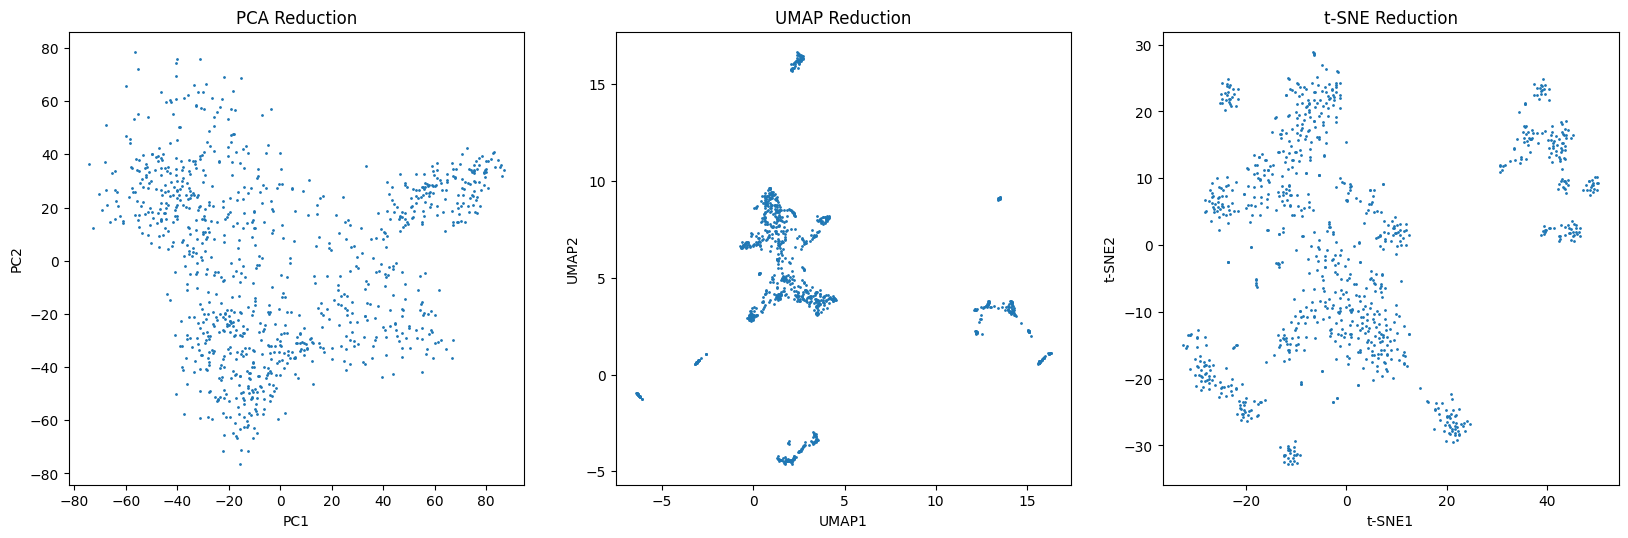
\includegraphics[width=\textwidth]{Images/default_dimred.png}
    \caption{PCA (left), UMAP (middle), and t-SNE (right) reduction using default parameters.}
    \label{fig:default_dimred}
\end{figure}

\vspace{-0.5cm}

A quick implementation with the default parameters of each technique gives some insight into the nature of the performance. As seen in Figure \ref{fig:default_dimred}, distinct regions of point clusters have been generated in both the UMAP and t-SNE plots. The PCA plot, however, does not show any distinct clusters and instead shows a large cloud of points with no discernible structure. Knowing that both UMAP and t-SNE are non-linear techniques, it can be deduced that perhaps linear methods, such as PCA, are not the most suitable dimensionality reduction approaches for this dataset.

In addition to the visual inspection of the plots, the runtime of each technique was also recorded when run on a machine with an Intel i7-8750H processor and 16 GB of RAM. The runtime of each technique is shown in Table \ref{tab:default_dimred}.

\begin{table}[H]
    \centering
    \begin{tabular}{|c|c|}
        \hline
        \textbf{Method} & \textbf{Runtime (s)} \\
        \hline
        PCA & 0.383  \\
        UMAP & 5.850 \\
        t-SNE & 3.916 \\
        \hline
    \end{tabular}
    \caption{Runtime of each technique using default parameters.}
    \label{tab:default_dimred}
\end{table}

\vspace{-0.5cm}

A point to note is that while both UMAP and t-SNE have generated distinct clusters, the clusters are not identical in shape or density. UMAP has produced denser clusters that are closer to the origin, while t-SNE has produced a similar amount of clusters that are more spread out, both in terms of point-to-point and cluster-to-cluster. To examine the non-linear techniques further, parameters of interest were changed in isolation to analyze their effect on the resulting plots. 

\subsubsection{UMAP Parameter Analysis}
A sequence of reductions with varying number of neighbors in UMAP is observed in Figure \ref{fig:UMAP_vary}.

\begin{figure}[H]
    \centering
    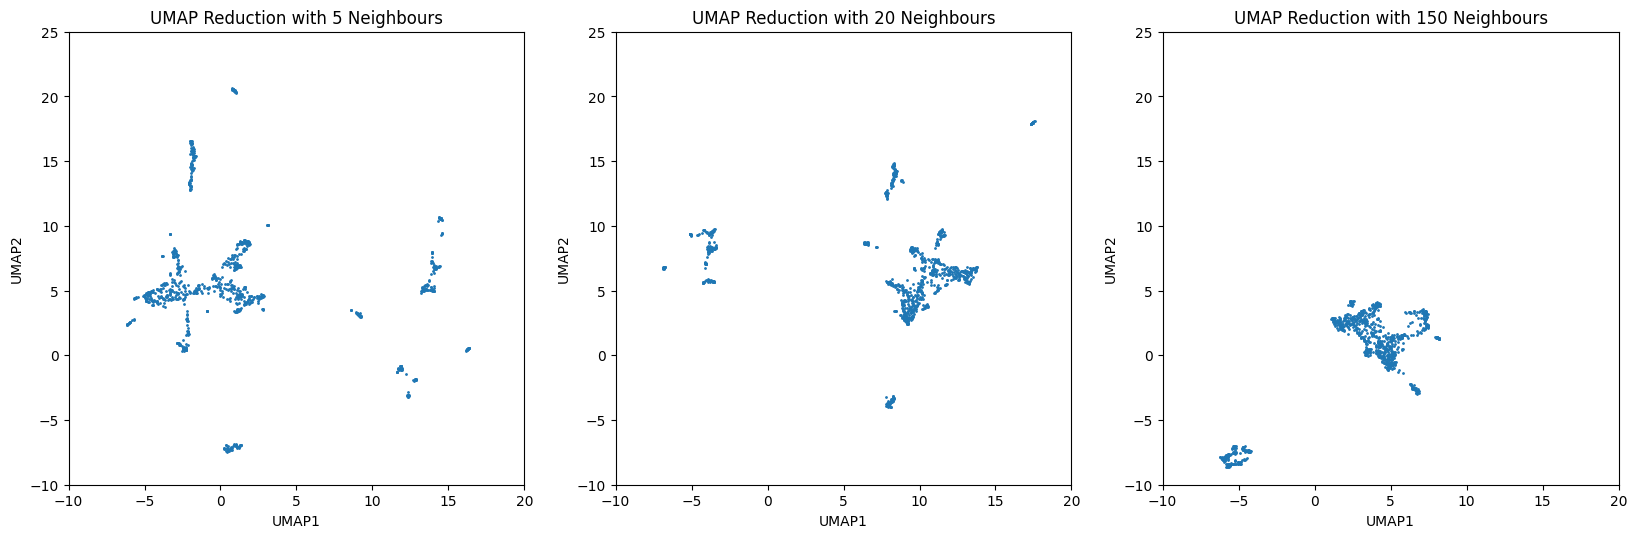
\includegraphics[width=\textwidth]{Images/UMAP_vary.png}
    \caption{UMAP reduction of the data varying the number of neighbors.}
    \label{fig:UMAP_vary}
\end{figure}

\vspace{-0.5cm}

Visually, adjusting the number of neighbors considered in a UMAP reduction provides a different insight into the relationships between data points. As seen in Figure \ref{fig:UMAP_vary}, the number of clusters identified by the algorithm decreases as the number of neighbors increases. It can be discerned then, that considering more neighbors captures broader trends in the data, while considering fewer neighbors captures more local trends.

A sequence of reductions with varying minimum distance in UMAP is observed in Figure \ref{fig:UMAP_vary2}.

\begin{figure}[H]
    \centering
    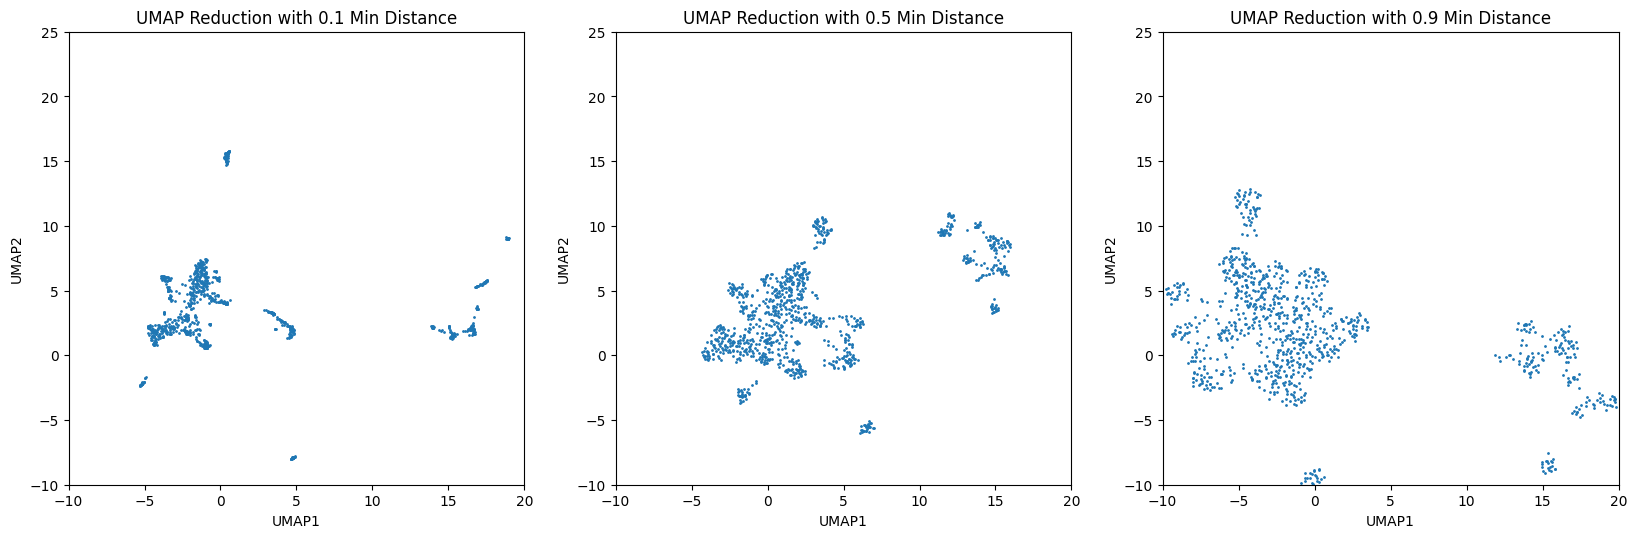
\includegraphics[width=\textwidth]{Images/UMAP_vary2.png}
    \caption{UMAP reduction of the data varying the minimum distance.}
    \label{fig:UMAP_vary2}
\end{figure}

\vspace{-0.5cm}

From inspection, the minimum distance parameter seems to have a spread effect on the clusters and data points. As the minimum distance increased, the clusters reduced in number and became more spread out. This is likely due to the fact that the minimum distance parameter is used to control the effective minimum distance between points. As the minimum distance increases, the algorithm is forced to spread out the clusters to meet the minimum distance requirement.

Depending on the objective of the dimensionality reduction, both the number of neighbors and the minimum distance parameters can be used to control the generalization of the algorithm. If the goal is to identify broad trends in the data, then a higher number of neighbors and a lower minimum distance should be used. If the goal is to identify local trends in the data, then a lower number of neighbors and a higher minimum distance should be used.

\subsubsection{t-SNE Parameter Analysis}
A sequence of reductions with varying perplexity in t-SNE is observed in Figure \ref{fig:TSNE_vary}.

\begin{figure}[H]
    \centering
    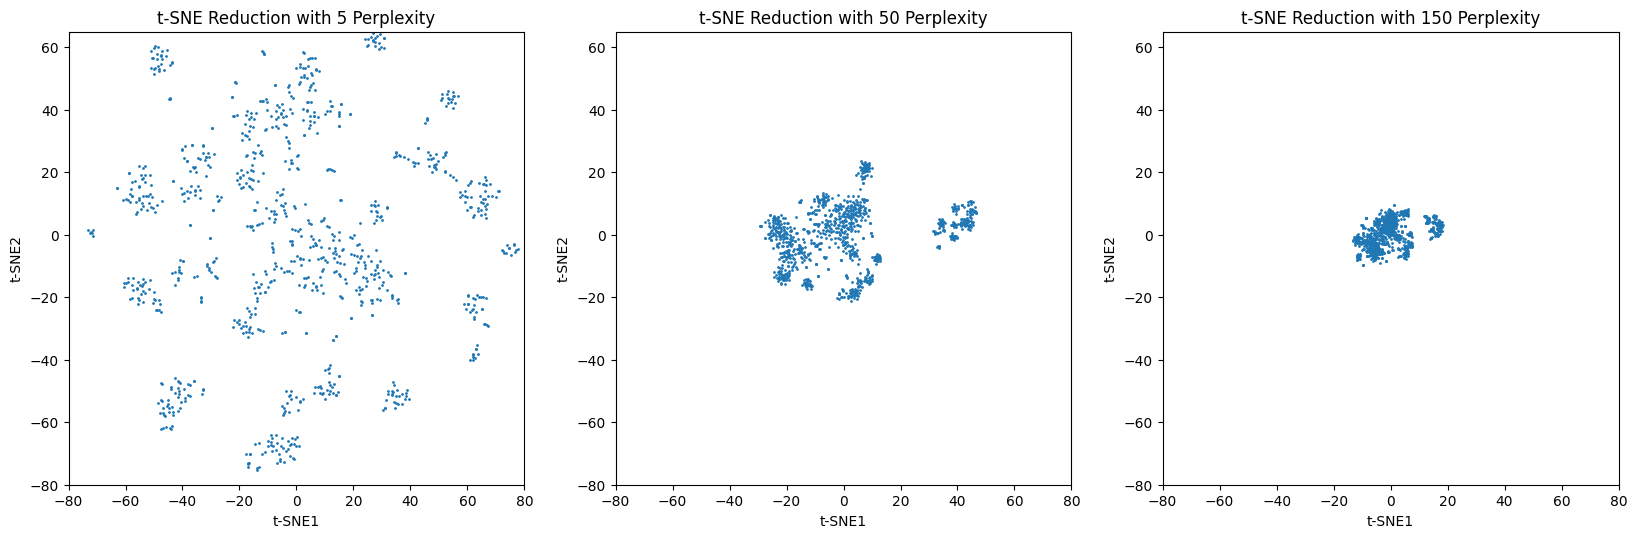
\includegraphics[width=\textwidth]{Images/t-sne_vary.png}
    \caption{t-SNE reduction of the data varying the perplexity.}
    \label{fig:TSNE_vary}
\end{figure}

\vspace{-0.5cm}

Similar to the number of neighbors parameter in UMAP, the perplexity parameter in t-SNE controls the number of neighbors considered when reducing the dimensionality of the data. As seen in Figure \ref{fig:TSNE_vary}, the number of clusters identified by the algorithm decreases as the perplexity increases. It can be similarly discerned then that considering more neighbors captures broader trends in the data, while considering fewer neighbors captures more local trends.

Again, depending on the objective of the dimensionality reduction, the perplexity parameter can be used to control the generalization of the algorithm. If the goal is to identify broad trends in the data, then a higher perplexity should be used. If the goal is to identify local trends in the data, then a lower perplexity should be used.

\subsection{Discussion of Results}
\begin{enumerate}
    \item \textbf{Do you see different clusters forming (visually)? How much correspondence exist between clusters that you find in different methods?}

    Different clusters formed visually in the UMAP and t-SNE plots. The clusters in the UMAP plot were denser and closer to the origin, while the clusters in the t-SNE plot were more spread out. The clusters in the PCA plot were not visually discernible.  

    Varying the parameters of both the UMAP and t-SNE algorithms resulted in different clusters being formed. The number of clusters identified by the algorithms decreased as the number of neighbors or perplexity increased. This is due to the fact that considering more neighbors or a higher perplexity captures broader trends in the data, while considering fewer neighbors or a lower perplexity captures more local trends. Therefore, the non-linear techniques are surely capable of producing high correspondence, but the parameters must be tuned to achieve this correspondence. However, neither UMAP nor t-SNE had correspondence with the PCA plot.

    \item \textbf{What is the difference between the three methods above? Use pros/cons to compare them against each other.}
    
    PCA is a fast algorithm (was the fastest of the three), is computationally efficient, scaled well with this large dataset, and is highly interpretable. However, PCA assumes that linear relationships are present in the data, and is therefore not suitable for datasets with non-linear relationships. In these cases, a loss of local structure can occur. It appears that the linear assumption did not hold particularly well with this dataset, as the PCA plot did not show any discernible preserved structure.

    UMAP is a non-linear, highly customizable, dimensionality reduction technique that is capable of reducing the dimensionality of a dataset while preserving the local and global structure of the data. In this implementation, UMAP was the slowest of the three algorithms as a result of its high degree of complexity. However, it was best suited for this dataset as it was able to capture the non-linear relationships in the data and produce dense clusters from the data capturing both local and global trends.

    t-SNE is another non-linear dimensionality reduction technique that was effective in identifying relationships in the gene expression data. Like UMAP, it appeared to be effective in preserving local structures in the data. Further, t-SNE was faster than UMAP, but could not generate clusters as dense on a 2D plot. However, like UMAP, t-SNE is tunable and can be used to capture local trends in the data effectively. 
\end{enumerate}

\section{Part 2: Clustering}

\begin{comment}
\subsection{Theory}
\subsubsection{Agglomerative Clustering}
Agglomerative clustering is a clustering approach that works by first partitioning a dataset into singleton clusters, and then iteratively merging the clusters together until there is only one cluster remaining \cite{mullner_modern_2011}. There are several parameters that govern the algorithm: linkage, distance metric, and, obviously, the number of clusters. Linkage refers to the method used to calculate the distance between clusters, while the distance metric refers to the method used to calculate the distance between points. 

\subsubsection{K-Means Clustering}
K-means clustering is a traditional unsupervised algorithm used to partition a dataset into $k$ clusters. The algorithm works by first initializing $k$ centroids, iteratively assigning each point to the cluster with the closest centroid, and then updating the centroids based on the new cluster assignments until a steady state is reached. The algorithm is sensitive to the initial centroid positions, and therefore, the algorithm is typically run multiple times with different initialization to ensure that the global minimum is reached.
\end{comment}

\subsection{Implementation}
The \verb|sk.learn.cluster.AgglomerativeClustering| function was used to implement agglomerative clustering. Initially, the function was used with its default parameters with the exception of the number of clusters, which was set to 3. With its default settings, the agglomerative clustering algorithm uses a ``ward'' linkage, which minimized the variance of clusters being merged, and Euclidean affinity.

The \verb|sklearn.cluster.KMeans| function was used to implement K-means clustering with a specification of 3 clusters. Given that the initial clusters are assigned randomly, the following results are based on an individual run of the algorithm and are therefore are not fully reproducible without setting a random seed.

\subsubsection{Jaccard Similarity with Default Parameters}
The computed clusters of each algorithm were compared using the Jaccard similarity metric implemented via the \verb|sklearn.metrics.jaccard_score| function. An iterative approach was conducted to compute the similarity of the nine permutations of the three algorithms. The results of this approach are shown in Table \ref{tab:jaccard_default}. Note that the rows represent the clusters computed by the agglomerative algorithm, while the columns represent the clusters computed by the K-means clustering algorithm.

\begin{table}[H]
    \centering
    \begin{tabular}{|c|c|c|c|}
        \hline 
        \diagbox{Agg.}{K-means} & \textbf{Cluster 1} & \textbf{Cluster 2} & \textbf{Cluster 3} \\
        \hline
        \textbf{Cluster 1} & 0.892 & 0.000 & 0.044 \\
        \textbf{Cluster 2} & 0.000 & 1.000 & 0.000 \\
        \textbf{Cluster 3} & 0.022 & 0.000 & 0.864 \\
        \hline
    \end{tabular}
    \caption{Jaccard similarity of the clusters using default parameters.}
    \label{tab:jaccard_default}
\end{table}

\vspace{-0.5cm}

The Jaccard similarity metric is a measure of the similarity between two sets. The metric is defined as the size of the intersection of the sets divided by the size of the union of the sets. In this case, the sets are the clusters identified by the algorithms. The Jaccard similarity metric is a value between 0 and 1, where 0 indicates no similarity and 1 indicates perfect similarity. From Table \ref{tab:jaccard_default}, it can be seen that the clusters identified by the algorithms are not identical, however there is a high degree of similarity. Note that the values were rounded to 3 decimal places for readability. 

\subsubsection{Rand Index with Default Parameters}
The computed clusters of each algorithm were compared using the Rand index metric implemented via the \verb|sklearn.metrics.adjusted_rand_score| function. Adjusting for 3 decimal places, the Rand-index of the two algorithms at default parameters was approximately \textbf{0.918}, on a scale from 0 to 1, with 1 indicating perfect correspondence.

\subsubsection{Adjusted Rand Index with Default Parameters}
The computed clusters of each algorithm were compared using the adjusted Rand index metric implemented via the \verb|sklearn.metrics.adjusted_rand_score| function. Adjusting for 3 decimal places, the adjusted Rand-index of the two algorithms at default parameters was approximately \textbf{0.825}, on a scale from -1 to 1, with -1 indicating disagreement, 0 indicating randomness, and 1 indicating a perfect correspondence.

Clearly, both indexes suggest that the clusters identified by the algorithms are not identical, however there is a high degree of similarity.

\subsection{Analysis of Agglomerative Clustering}
Agglomerative clustering was implemented separately with average linkage and Euclidean and cosine distance metrics. A Jaccard similarity analysis of this implementation are shown in Table \ref{tab:average_agglo}.

\begin{table}[H]
    \centering
    \begin{tabular}{|c|c|c|c|}
        \hline 
        \diagbox{Euclidean}{Cosine} & \textbf{Cluster 1} & \textbf{Cluster 2} & \textbf{Cluster 3} \\
        \hline
        \textbf{Cluster 1} & 1.000 & 0.000 & 0.000 \\
        \textbf{Cluster 2} & 0.000 & 1.000 & 0.000 \\
        \textbf{Cluster 3} & 0.000 & 0.000 & 1.000 \\
        \hline
    \end{tabular}
    \caption{Jaccard similarity of the clusters using average linkage and Euclidean and cosine distance.}
    \label{tab:average_agglo}
\end{table}

\vspace{-0.5cm}

Interestingly, the clusters produced by the average linkage algorithm are identical regardless of the distance metric used. Correspondingly, the Rand-Index and adjusted Rand-Index were found to be \textbf{1.0}. Therefore, it can be concluded that the clusters produced by the average linkage algorithm are identical regardless of the distance metric used for this dataset.

A further analysis was conducted to examine the similarity between the clusters produced by the average linkage algorithm and the K-means algorithm. The results of this analysis are shown in Table \ref{tab:agglo_euc}.

\begin{table}[H]
    \centering
    \begin{tabular}{|c|c|c|c|}
        \hline 
        \diagbox{Agg.}{K-means} & \textbf{Cluster 1} & \textbf{Cluster 2} & \textbf{Cluster 3} \\
        \hline
        \textbf{Cluster 1} & 0.475 & 0.002 & 0.000 \\
        \textbf{Cluster 2} & 0.174 & 0.000 & 0.000 \\
        \textbf{Cluster 3} & 0.349 & 0.000 & 0.017 \\
        \hline
    \end{tabular}
    \caption{Jaccard similarity of the clusters using average linkage and K-means.}
    \label{tab:agglo_euc}
\end{table}

\vspace{-0.5cm}

In addition to the Jaccard similarity metric, the Rand index and adjusted Rand index were also computed. The Rand index was approximately \textbf{0.382}, while the adjusted Rand index was approximately \textbf{0.0}.

Average linkage clustering with Euclidean and cosine distance metrics produced clusters that were not similar to the clusters produced by the K-means algorithm. In retrospect, this aligns well with expectation. Both ward linkage and K-means techniques aim to minimize cluster variance and create clusters that are of roughly equal shape and size. Average linkage techniques, on the other hand, take into account the mean distance between all points in neighboring clusters. As a result, clusters formed can be of abnormal shapes and sizes. 

\subsubsection{Analysis of Agglomerative Clustering on Subsets of the Data}
The agglomerative clustering algorithm was implemented on subsets of the data to observe why both Euclidean and cosine distance metrics produced identical clusters. 

First, subsets of the data were created by only including randomly selected features from the data. The agglomerative clustering algorithm was then implemented on the subsets of the data using Euclidean and cosine distance metrics. The results of this analysis are shown in Table \ref{tab:agglo_euc_sub}.

\begin{table}[H]
    \centering
    \begin{tabular}{|c|c|c|}
        \hline 
        \textbf{Number of Features} & \textbf{Rand Score} & \textbf{Adjusted Rand Score} \\
        \hline
        25 & 0.996 & 0.831 \\
        100 & 0.996 & 0.855 \\
        200 & 0.998 & 0.922 \\
        300 & 1.0 & 1.0 \\
        \hline
    \end{tabular}
    \caption{Similarity of the clusters using average linkage and Euclidean and cosine distance on feature subsets of the data.}
    \label{tab:agglo_euc_sub}
\end{table}

\vspace{-0.5cm}

Next, subsets of the data were created by only including randomly selected samples from the data. The agglomerative clustering algorithm was then implemented on the subsets of the data using Euclidean and cosine distance metrics. The results of this analysis are shown in Table \ref{tab:agglo_euc_sub2}.

\begin{table}[H]
    \centering
    \begin{tabular}{|c|c|c|} 
        \hline
        \textbf{Number of Samples} & \textbf{Rand Score} & \textbf{Adjusted Rand Score} \\
        \hline
        25 & 1.0 & 1.0 \\
        100 & 1.0 & 1.0 \\
        200 & 1.0 & 1.0 \\
        300 & 1.0 & 1.0 \\
        \hline
    \end{tabular}
    \caption{Similarity of the clusters using average linkage and Euclidean and cosine distance on sample subsets of the data.}
    \label{tab:agglo_euc_sub2}
\end{table}

\vspace{-0.5cm}

From these observations a more clear understanding of the gene expression data can be conveyed. Here, it is seen that removing samples does not result in the two distance metrics producing different clusters. However, removing features does. This could be related to the dimensionality reduction analysis done prior. 

Both UMAP and t-SNE reduction showed that tight clusters form in the data at lower dimensions. This sense of structure causes Euclidean and cosine distance metrics to perform similarly - it is not until the structure itself is modified that these two distance metrics will disagree with each other. In this case, removing samples does not seem to change the structure of the data enough to note any differences. However, removing features (until there are only approx. 300) changes the dimensionality and structure of the data enough to highlight the difference in these two clustering methods. The clusters produced by the two distance metrics are still very similar, but not identical.

\section{Regression}

\subsection{Regularization Analysis}
In this section, target data was introduced to the dataset in the form of drug response data. The drug response vector was aligned with the gene expression data, with all instances being aligned with the same drug response value, and instances with no drug response data being removed. The feature data was then normalized using the \verb|sklearn.preprocessing.StandardScaler| function for faster convergence of the regression model.

A LASSO regression model, which is a linear model with L1 regularization, was then fit to the data using the \verb|sklearn.linear_model.Lasso| function. The model was fit using a range of alpha values in [0.01, 0.1, 0.3, 0.5, 0.9], where the optimal weight vector is given by:
\begin{align*}
    w^* = \min_w \frac{1}{2n_{samples}}||Xw-y||_2^2 + \alpha||w||_1
\end{align*}

An analysis was done to examine how the value of alpha affects the number of features selected by the LASSO regression model. This was implemented by iterating over the alpha values and recording the number of non-zero coefficients in the weight vector. The results of this analysis are shown in Figure \ref{fig:lasso_alpha}.

\begin{figure}[H]
    \centering
    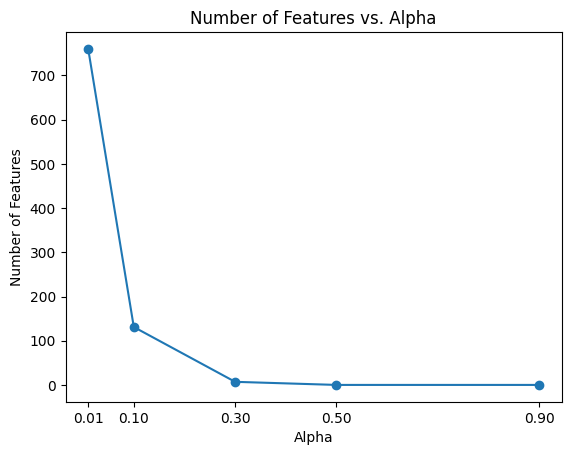
\includegraphics[width=0.6\textwidth]{Images/regularization.png}
    \caption{Number of non-zero coefficients in the weight vector as a function of alpha.}
    \label{fig:lasso_alpha}
\end{figure}

The results are also shown in Table \ref{tab:lasso_alpha}.

\begin{table}[H]
    \centering
    \begin{tabular}{|c|c|}
        \hline 
        \textbf{Alpha} & \textbf{Number of Non-Zero Coefficients} \\
        \hline
        0.01 & 760 \\
        0.1 & 131 \\
        0.3 & 7 \\
        0.5 & 0 \\
        0.9 & 0 \\
        \hline
    \end{tabular}
    \caption{Number of non-zero coefficients in the weight vector as a function of alpha.}
    \label{tab:lasso_alpha}
\end{table}

\vspace{-0.5cm}

As alpha increases, the sparsity of the solution increases dramatically. This is conventional with theory, as more weight is given to the L1 norm penalty and thus the optimal solution will be more sparse. With this dataset, it is seen that an alpha value of 0.5 results in a weight vector with no non-zero coefficients. 

\subsection{Nested Cross-Validation}
Nested cross-validation is a technique used for robustly evaluating the performance of machine learning models while simultaneously optimizing the hyperparameters associated with the models. 

Initially, inner and outer loop cross-validation (CV) folds are established employing stratification to ensure balanced representation. In this case, it was specified that the outer loop was to have 4 folds, while the inner loop was to have 3. Subsequently, a parameter grid is defined to be iterated over during hyperparameter optimization, which occurs in the inner loop of the CV process. In this case, the hyperparameter alpha was tested at values [0.01, 0.1, 0.3, 0.5, 0.9].

In the outer loop, the data is partitioned into 4 distinct training (75\% of the data) and test sets (25\% of the data). Within each outer fold, the training data is partitioned again into 3 folds of training (66\%) and validation sets (33\%). The inner loop is used to compare the performance of each model at the specified hyperparameter values. In this case, it was known that the LASSO estimator was to be used, so correspondingly model performance was evaluated in the inner loop using MSE. 

The alpha value that results in the lowest MSE in the inner loop cross validation is then used in the model to be evaluated in the outer loop. The model is re-fit on the entire outer fold training set, and evaluated on the unseen test set using MSE and Spearman Rank Correlation. This process is repeated for each outer fold, resulting in 4 MSE and Spearman Rank Correlation values. The average of these values is then taken as the final performance metric for the model.

\subsection{Implementation}
The procedure outlined above was implemented in Python using Scikit-learn. 

The \verb|sklearn.model_selection.KFold| method was used to define the outer and inner loops desired. First, the feature data was split via the outer loop object and then a for-loop was constructed to iterate over each outer fold. Within each outer fold, the data was partitioned into train and validation subsets to be used in the inner loops. 

The \verb|sklearn.model_selection.GridSearchCV| object parameterized by a LASSO estimator, the parameter grid, and the inner loop fold object was then used to perform the inner loop CV process. The grid search object automatically optimized the hyperparameters of the estimator based on the inner loop CV, refit the model on the entire outer fold training set, and then was able to return various metrics such as the optimal hyperparameter value and the best estimator model. The best estimator was then used to predict the test set of the outer fold with its performance evaluated by MSE and Spearman Rank Correlation. 

This process was repeated for each outer fold, and the average MSE and Spearman Rank Correlation were computed. Note that the Spearman Rank Correlation was computed using the \verb|scipy.stats.spearmanr| function.

\subsection{Cross-Validation Results}
The results of the nested cross-validation process at each outer loop fold are shown in Table \ref{tab:regression_results}.

\begin{table}[H]
    \centering
    \begin{tabular}{|c|c|c|c|c|}
        \hline
        Outer Fold & Alpha & Mean Squared Error & Spearman Correlation & p-value \\
        \hline
        1 & 0.1 & 2.308 & 0.323 & $1.1 \times 10^{-6}$ \\
        2 & 0.1 & 2.258 & 0.341 & $2.0 \times 10^{-7}$ \\
        3 & 0.1 & 2.93 & 0.317 & $1.8 \times 10^{-6}$ \\
        4 & 0.1 & 2.306 & 0.344 & $2.0 \times 10^{-7}$ \\
        \hline
    \end{tabular}
    \caption{Results of the nested cross-validation process.}
    \label{tab:regression_results}
\end{table}

\vspace{-0.5cm}

The Spearman Rank Correlation at each outer loop fold was found to be statistically significant at a significance level of less than 0.05. Thus, the average MSE and Spearman Rank Correlation of a LASSO regression model were found to be \textbf{2.451} and \textbf{0.331} respectively.

Each inner loop CV observed that the optimal alpha value was 0.1. Given the consistency, it seems that the optimal alpha value is not sensitive to the folds in the training data. 

\subsection{Comparison to Baseline}
To further evaluate the LASSO regression model, its performance in MSE was compared to some basic baseline models - a mean estimator and a median estimator. The mean estimator simply predicts the mean of the training data for all test instances, while the median estimator simply predicts the median of the training data for all test instances. The dummy models were evaluated using the same outer loop CV process as the LASSO regression model, and the average MSE was computed. Note that no Spearman Rank Correlation was computed for the dummy models as they predict a constant value for all test instances.

The results of this comparison are shown in Table \ref{tab:regression_baseline}.

\begin{table}[H]
    \centering
    \begin{tabular}{|c|c|c|}
        \hline
        Dummy Model & MSE & Spearman Rank Correlation \\
        \hline
        Mean & 2.780 & NaN \\
        Median & 2.798 & NaN \\
        \hline
    \end{tabular}
    \caption{Results of the dummy models.}
    \label{tab:regression_baseline}
\end{table}

\vspace{-0.5cm}

The LASSO regression model was found to outperform both the mean and median dummy models in MSE and Spearman Rank Correlation. 

\newpage

\bibliographystyle{IEEEtran}
\bibliography{references}

\end{document}
